%TODO synthèse
%TODO glossaire et bibliographie etc ..

%%%%%%%%%%%%%%%%%%%%%%%%%%%%%%%%%%%%%%%%%%%%%%%%%%%%%%%%%
%                      Préambule                        %
%%%%%%%%%%%%%%%%%%%%%%%%%%%%%%%%%%%%%%%%%%%%%%%%%%%%%%%%%

%%%%%%%%%%%%%%%%%%%%%%%%%%%%%%%%%%%%%%%%%%%%%%%%%%%%%%%%%%%%%%%%%
%                      Préambule type                          %
%%%%%%%%%%%%%%%%%%%%%%%%%%%%%%%%%%%%%%%%%%%%%%%%%%%%%%%%%%%%%%%%



\def\changemargin#1#2{\list{}{\rightmargin#2\leftmargin#1}\item[]}
\let\endchangemargin=\endlist 

%%%%%%%%%%%%%%%%%% Classe dudit Document %%%%%%%%%%%%%%%%%%%%%%%
\documentclass[a4paper,12pt,openany]{report} % sert à définir des propriétés e base sur les articles
% Autre paramètres connnus: 	*book => pour de vrais livres
%				*article pour des artiles dans des revues scientifiques, des présentations, des rapports courts, des documentations, des invitation etc....
%				*report por des rapports plus long contenant plusieurs chapitres, des petits livres, des thèses
%				*Slides pour des transparants
%				*foiltex
% Option: Xpt taille de la police,  4apaper/letterpaper/a5paper/b5paper/executivepaper, fleqn, leqno, titlepage/notitlepage indique si une nouvelle page doit être commencée après le titre du document, twocolumn,twoside/oneside,



%%%%%%%%%%%%%%%%%%%%%%%% Package %%%%%%%%%%%%%%%%%%%%%%%%%%%%%%%
\usepackage{doc}% permet de documenter des programmes (cf doc.dtx]
\usepackage{exscale} % fournit des version de taille de caractère que LaTeX va utiliser (cf ltexscale.dtx)
\usepackage{fontenc} % spécifie le codage des police de caractère que LaTeX va utiliser (cf ltoutenc.dtx)
%\usepackage[latin]{inputenc} %Autorise les caractères acentués
\usepackage{ifthen} % fournit des commandes de conditions (cf ifthen.dtx)
\usepackage{latexsym} %permet l'utilisation de la police des symboles LaTeX
\usepackage{makeidx} %fournit des commandes pour réaliser un index
\usepackage{syntonly} % analyse le doc sans le formater
\usepackage[T1]{fontenc}
\usepackage[utf8x]{inputenc} 
%\usepackage[utf8]{inputenc}% permet de spécifier le codeage des caractère utiliser dans le source.
\usepackage[english,francais]{babel}
%\usepackage{asmath} %Fonctions servant à l'écriture mathématique
\usepackage{xspace} %Fonctions permettant d'introduire des espaces
\usepackage{xargs} %Permet d'utiliser de définir plus simplement des fonctions
\usepackage{trace}%Permet d'utiliser des traces de debbug
\usepackage{show2e}% debbug
\usepackage[pdftex]{graphicx}
\usepackage{hyperref}

%%%%%%%%%%%%%%%%% Style du pied de page %%%%%%%%%%%%%%%%%%%%%%%%

\pagestyle{plain}% imprime le numéro de page au milieu du pied de page
%\pagestyle{heading}%imprime le titre du chapitre courant et le numéro dans l'en tête et laisse le pied de page vide.
%\pagestyle{empty}% laisse l'en tête et le pied de page vide


%Nota bene: On peut changer le pied de page en court en utilisant \thispagestyle


%%%%%%%%%%%%%%%%% Césure   %%%%%%%%%%%%%%%%%%%%%%%%

\hyphenation{FORTRAN}
\hyphenation{An-ti-cons-ti-tu-tion-nel-le-ment}

%%%%%%%%%%%%%%%% Citation Environement %%%%%%%%%%%%

\newsavebox{\nomepigraphe}
\newenvironment{epigraphe}[1]
	{% clause begin
	\vspace*{-1.5cm}%
	\small\sffamily% mise en évidence
	\savebox{\nomepigraphe}{#1}% une boîte pour sauvegarder
	% l’ origine de la citation
	\slshape% tout est penché
	\begin{changemargin}{0pt}{-2cm}% on se met au large
	\begin{flushright}}% tout est poussé à droite
	{% clause end
	\\[4pt]\usebox{\nomepigraphe}.% insertion de l’origine
	\end{flushright}%
	\end{changemargin}\par\vspace*{0.6cm}}

%
\input ./preambule.tex %sans saut de ligne


%%%%%%%%%%%%%%Titre%%%%%%%%%%%%%%%%%%%%%%%%%%%%%%%%%%%%
\title{ Projet de 3 année à l'INSA Centre Val de Loire } % Titre du document
\author{BAIZ Mamoune && BAIZ Mamoune} % Auteur
\date{\today} % Date de création


%%%%%%%%%%%%%%%%%%%%%%%Debut Doc%%%%%%%%%%%%%%%%%%%%%%%
\begin{document} % Début du document
%%%%%%%%%%%%%%%%%%%%%%Page de Garde%%%%%%%%%%%%%%%%%%%%
{
\begin{titlepage}
  \begin{sffamily}
  \begin{center}

    % Upper part of the page. The '~' is needed because \\
    % only works if a paragraph has started.
    
\includegraphics[scale=0.5]{Images/png/insa_logo.png}~\\[1.5cm]

    \textsc{\LARGE Institut National des Sciences Appliquées  Centre Val de Loire }\\[2cm]

    \textsc{\Large Rapport de projet 3\up{ème} année option 2SU}\\[1.5cm]

    % Title
%    \HRule \\[0.4cm]
    { \huge \bfseries Domotique\\[0.4cm] }

%    \HRule \\[2cm]
    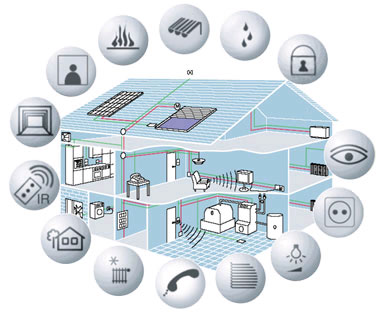
\includegraphics[scale=0.5]{Images/jpg/domotic.jpg}
    \\[2cm]

    % Author and supervisor
    \begin{minipage}{0.4\textwidth}
      \begin{flushleft} \large
        BAIZ Mamoune et MUNIER Marc \\
        Promo 2016\\
      \end{flushleft}
    \end{minipage}
    \begin{minipage}{0.4\textwidth}
      \begin{flushright} \large
        \emph{Encadrant :} M. Briffaut\\
      \end{flushright}
    \end{minipage}

    \vfill

    % Bottom of the page
    {\large 9 Février 2016}

  \end{center}
  \end{sffamily}
\end{titlepage}
}
%%%%%%%%%%%%%%%%%%%%%%%Page Vierge%%%%%%%%%%%%%%%%%%%%
\newpage



%%%%%%%%%%%%%%%%%%%%% Remerciment %%%%%%%%%%%%%%%%%%%%
\newpage
\section*{Remerciement}
Je tiens à remercier Mr Briffaut pour sa investissement 
%TODO
\clearpage
%%%%%%%%%%%%%%%%%%%%%Résumé%%%%%%%%%%%%%%%%%%%%%%%%%%%
\section*{Résumé}
Ce rapport présente mon travail et les enseignements acquis lors de mon stage de deuxième année d'école d'ingénieurs au seins du Centre technique de la Gendarmerie nationale. 

%%%%%%%%%%%%%%%%%%%%%table des matières%%%%%%%%%%%%%%%
\newpage
\tableofcontents
\clearpage

%%%%%%%%%%%PLAN
%
%I) Introduction ( comment on a fait ce projet, en quoi il consiste, les enjeux )
%II)	Presentation du résultat final.
%		A)	les outils ( raspberry + capteur)
%		B)	le Logiciel (domoticz)
%		C)	l'application
% 
%III)	Comment le mettre en place 
%IV)	présentation appronfondie des composants.
%V)		Nos diffficultés difficulté
%VII)	Conclusion
%
%
%Ne pas oublier le glossaire.
%
% chaque partie est à ecrire dans un fichier indépandant du main
% il suffit de rajouter la ligne suivante pour inclure ces écrits
%\input ./maPartie.tex %sans saut de ligne
%
%%%%%%%%%%%%%%%%%%%


%%%%%%%%%%%%%%%%%%%%%%%%%%%%%%%%%%%%%%%%%%%%%%%%%%%%%%
\section{Introduction}

%%%%%%%%%%%%%%%%%%%%%%%%%%%%%%%%%%%%%%%%%%%%%%%%%%%%%%%
\end{document}
